\documentclass[10pt,a4paper]{ULBreport}
\usepackage[utf8]{inputenc}
\sceau{Images/sceauULB.jpg}
\graphicspath{ {./Images/} }
\usepackage{multirow}
\usepackage{listings}
\usepackage{color} 
\usepackage{setspace} 
\usepackage{amsmath}
\usepackage{hyperref}
\usepackage{pdfpages}
\usepackage{biblatex}
\usepackage{floatrow}
\usepackage{subcaption} 
\usepackage{siunitx}
\usepackage[many]{tcolorbox}
\usepackage{multirow}
\usepackage{listings}
\usepackage[dvipsnames]{xcolor}
\usepackage{fancyvrb}

\usepackage{xstring}
\usepackage{etoolbox}

% Colors


% BOXES FOR QUESTIONS

\newtcolorbox{questionBox}[2][]{
    fontupper=\bf,
    boxrule=1.5pt,
    colframe= black, % frame color
    fonttitle=\itshape,
    attach boxed title to top left={yshift=-0.3\baselineskip-0.4pt,xshift=2mm},
    title= #2,#1,
    enhanced,
    }

\newtcolorbox{bonusQuestionBox}[2][]{
    fontupper=\bf,
    boxrule=1.5pt,
    colframe= BlueViolet, % frame color
    colback=Periwinkle,
    coltitle=white,
    fonttitle=\itshape,
    attach boxed title to top left={yshift=-0.3\baselineskip-0.4pt,xshift=2mm},
    boxed title style={colback=Violet},
    title= #2,#1,
    enhanced,
    }





\begin{document} 


	\titleULB{
	title={Report Lab 1 \\ Dynamic Routing},
    studies={IRELE - MA1 Electrical Engineering},
    course ={ELEC-H417},
    author={\textit{Authors :} \\ Amaury ARICO \\ Alexis BOLLENGIER \\ Emmeran COLOT \\Sefa GÖNEN  },
    date={\textbf{Academic year :} \\ 2024 - 2025},
    teacher={\textit{Professor : } \\ Jean-Michel DRICOT \\\textit{Assistant : } \\ Navid LADNER },
    logo={Images/logo-polytech.jpg},
    manyAuthor
	}

\chapter{Mission 0 - Initial Topology Setup}

\begin{figure}[H]
    \caption{Initial topology}
    \centering
    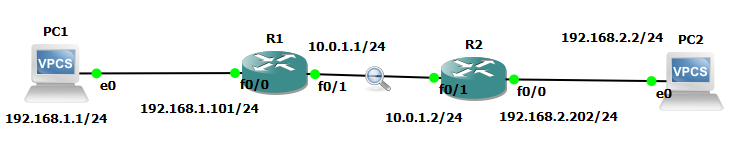
\includegraphics[width=0.7\textwidth]{topology.png}
    \label{topo}
\end{figure}


\section{Bonus question - Lost packet}

\begin{bonusQuestionBox}{Lost packet}
    Do you observe something special with the first (or two firsts) packet of the first ping command ? If yes, what is it and why ? (Wireshark could help)
\end{bonusQuestionBox}


% RESPONSE HERE

We can't ping devices at a distance $\geq 2$ because the routers don't know how to reach these devices (addresses not in the routing table).

Here are some screenshots proving it :

\begin{figure}[H]
    \caption{Ping from PC1 (192.168.1.1) to R1 (192.168.1.101)}
    \centering
    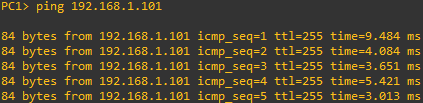
\includegraphics[width=0.7\textwidth]{pingPC1R1.png}
    \label{pingPC1R1}
\end{figure}

\begin{figure}[H]
    \caption{Ping from PC1 (192.168.1.1) to PC2 (192.168.2.2)}
    \centering
    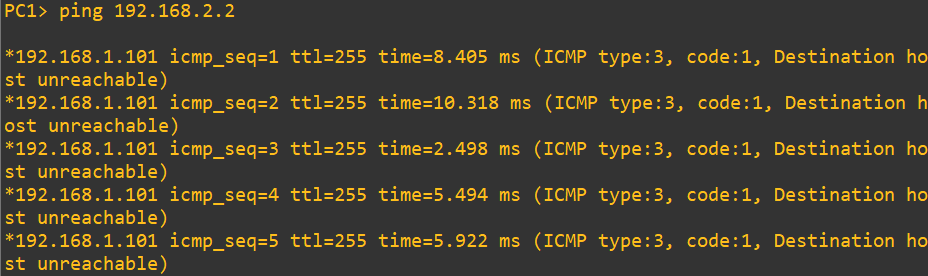
\includegraphics[width=0.7\textwidth]{pingPC1PC2.png}
    \label{pingPC1PC2}
\end{figure}

\begin{figure}[H]
    \caption{Routing table of R1}
    \centering
    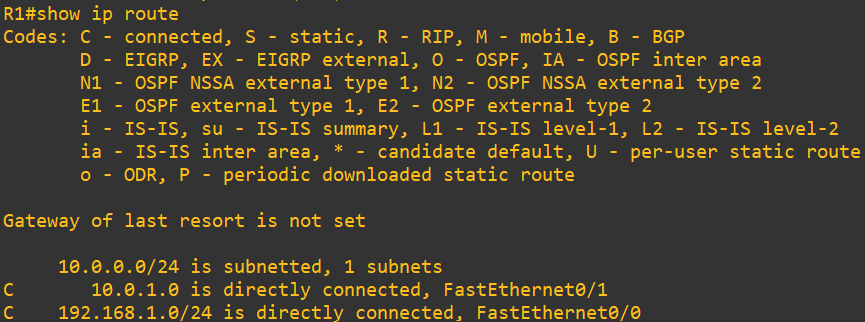
\includegraphics[width=0.7\textwidth]{routeRC1.png}
    \label{routeR1}
\end{figure}

\begin{figure}[H]
    \caption{Routing table of R2}
    \center
    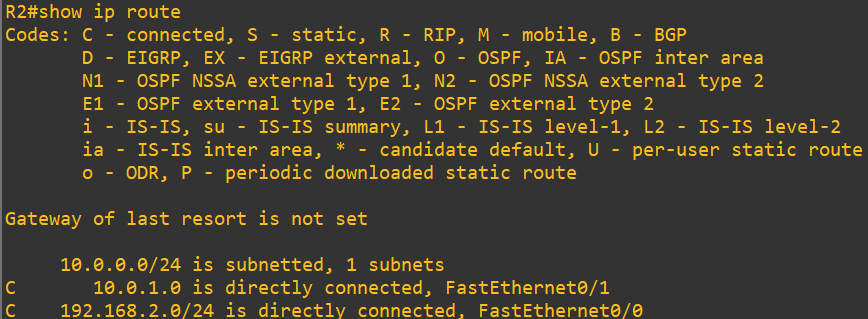
\includegraphics[width=0.7\textwidth]{routeRC2.png}
    \label{routeR2}
\end{figure}


% question : quand je fais ping PC1 -> R2, mon routeur R1 sait où il doit envoyer le ping (je reçois par wireshark le message ICMP)
% Mais le request de ping fail car R2 ne sait pas où envoyer la réponse (pas dans sa table de route)
% Donc pourquoi est-ce qu'on peut pas prendre le chemin inverse pour renvoyer la réposne ?
% Le packet ne contient peut être pas la route prise (sauf si on active l'option record route)



\chapter{Mission 1 - Configuring RIPv2}

\section{Question - Netmask adaptation}

\begin{questionBox}{Netmask adaptation}
    What should be the netmask to achieve this and why ?
\end{questionBox}


% Response here


No we can't ping from \textbf{PC1 to PC2}/PC2 to PC1 because the router \textbf{R1}/R2 doesn't know how to access \textbf{PC2}/PC1 (no routing information).



To solve this, we just need to configure the RIP protocol for R2. After configuring it, we can ping and the routing tables are updated :

\begin{figure}[H]
    \caption{Routing table of R1 after configuring RIPv2}
    \center
    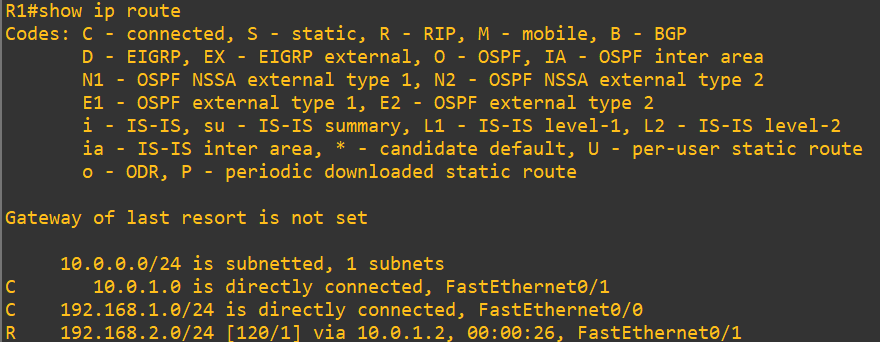
\includegraphics[width=0.7\textwidth]{routeR1RIP.png}
    \label{routeR1rip}
\end{figure}

\begin{figure}[H]
    \caption{Ping from PC1 to PC2}
    \center
    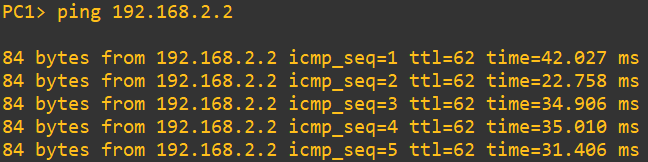
\includegraphics[width=0.7\textwidth]{pingPC1PC2RIP.png}
    \label{pingPC1PC2rip}
\end{figure}




\section{Question - Wireshark : What's Hiding in the RIP Packets?}

\begin{questionBox}{Wireshark : What's Hiding in the RIP Packets?}
    At what frequency RIP packets are send ? Is it send only once, periodic (and if so, at which frequency), sporadic (i.e. randomly) ? 
    What interesting information do you find in those packets (Put a Wireshark screenshot in your report and highlight these information on it) ?
\end{questionBox}


% Response here

The RIP packets are sent periodically, approximately every 30 seconds (see figure \ref{ripfreq}).

\begin{figure}[H]
    \caption{Wireshark screenshot. Listening to packets between R1 and R2 (subnet 10.0.1.0/24). Filtered to show packets sent by R1}
    \center
    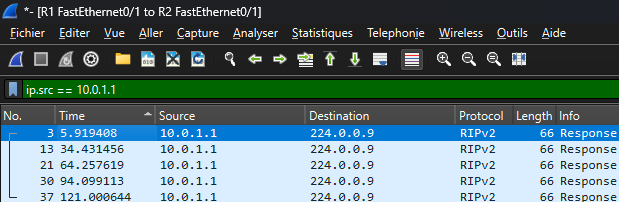
\includegraphics[width=0.7\textwidth]{RIPFreq.png}
    \label{ripfreq}
\end{figure}

The figure \ref{ripinfo} shows the content of the RIP packet. We can find in it \footnote{Information on the fields found from this website : \url{infocenter.nokia.com/public/7750SR222R1A/index.jsp?topic=/com.nokia.Unicast_Guide/rip_packet_form-ai9exj5yo9.html}} :

\begin{itemize}
    \item \textbf{IP address} : IP address of the network that the router serves (in this case R1 serves 192.168.1.0) 
    \item \textbf{Netmask} : The subnet mask of that network (in this case /24)
    \item \textbf{Next hop} : The IP address of the next router along the path to destination (0.0.0.0 means that the network 192.168.1.0/24 is directly connected to R1)
    \item \textbf{Metric} : The number of hops to the destination (1 in this case)
\end{itemize}

\begin{figure}[H]
    \caption{Wireshark screenshot. Listening to packets between R1 and R2. The content of one RIP packet sent by R1 is shown in the bottom left}
    \center
    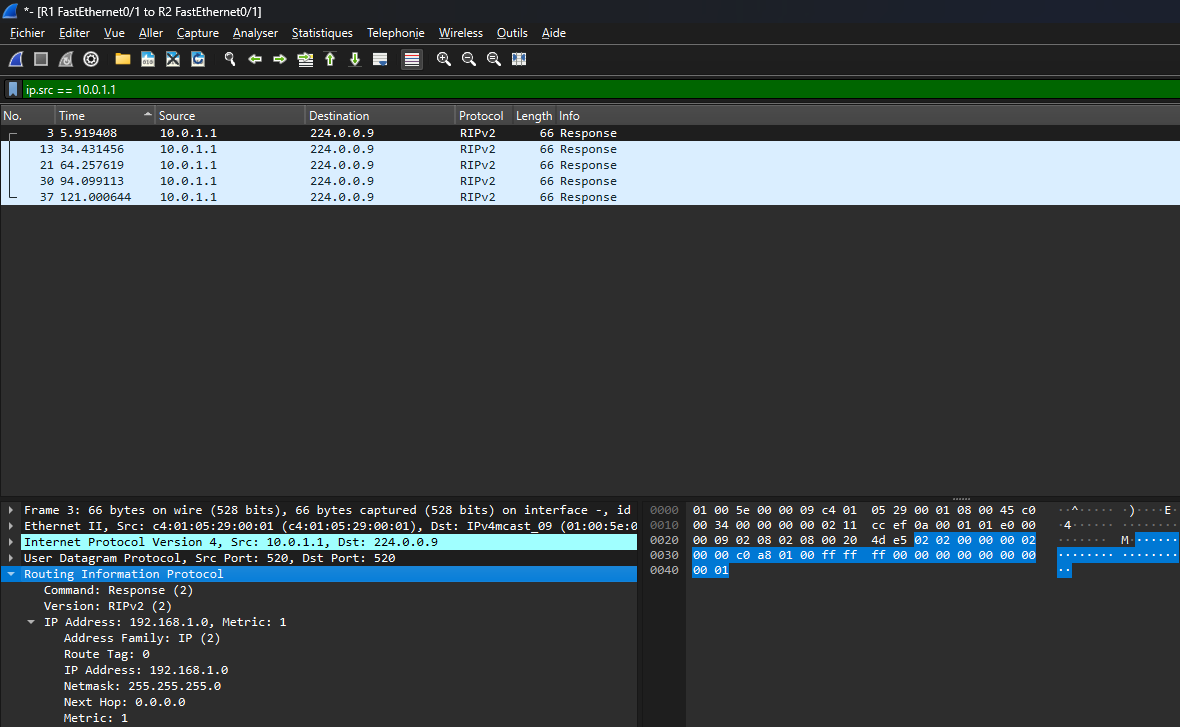
\includegraphics[width=0.7\textwidth]{RIPInfo.png}
    \label{ripinfo}
\end{figure}


\section{Bonus question - One-way communication}

\begin{bonusQuestionBox}{One-way communication}
    What can you do to make a one way communication (i.e. ping PC1→PC2 works but not PC2→PC1) ?
\end{bonusQuestionBox}


% Response here

If we want to do PC1 $\rightarrow$ PC2, we need to remove the subnet of PC1 (192.168.1.0) from the RIP database of R1. So the result is that my router R1 doesn't share the fact that it serves the network 192.168.1.0 but it receives the information from R2 that a network 192.168.2.0 exists. 

Command to do that :

\begin{lstlisting}[language=bash]
    R1#conf t
    R1(config)#router rip
    R1(config-router)#version 2
    R1(config-router)#no network 192.168.1.0
    R1(config-router)#end
    R1#write    
\end{lstlisting}

Results :

\begin{figure}[H]
    \caption{Routing table of R1 after removing the network 192.168.1.0 from the RIP database of R1}
    \center
    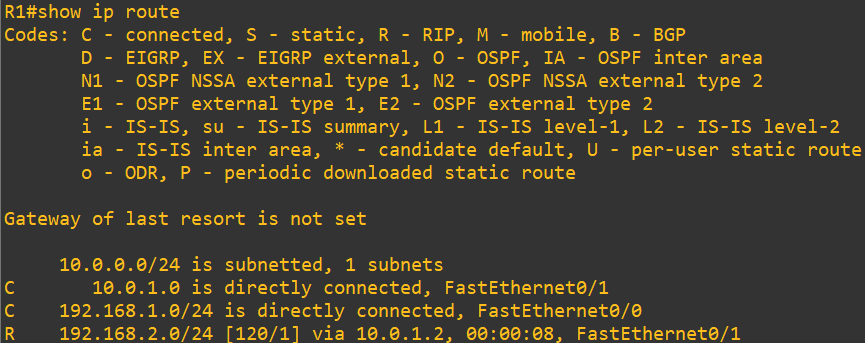
\includegraphics[width=0.7\textwidth]{routeR1SERIAL.png}
    \label{routeR1se}
\end{figure}

\begin{figure}[H]
    \caption{Routing table of R2 after removing the network 192.168.1.0 from the RIP database of R1}
    \center
    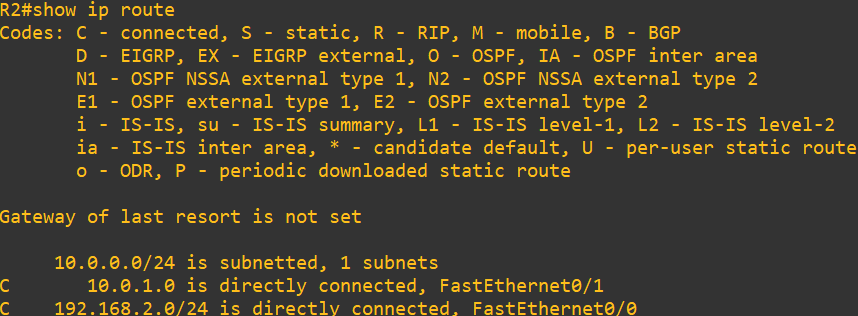
\includegraphics[width=0.7\textwidth]{routeR2SERIAL.png}
    \label{routeR2se}
\end{figure}

\begin{figure}[H]
    \caption{Ping from PC1 to PC2. Timeout because no response from PC2 (one way communication PC1 $\rightarrow$ PC2) }
    \center
    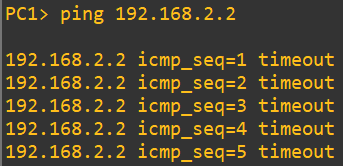
\includegraphics[scale=0.8]{pingPC1PC2SERIAL.png}
    \label{pingPC1PC2se}
\end{figure}

\begin{figure}[H]
    \caption{Ping from PC2 to PC1. Unreachable (one way communication PC1 $\rightarrow$ PC2)}
    \center
    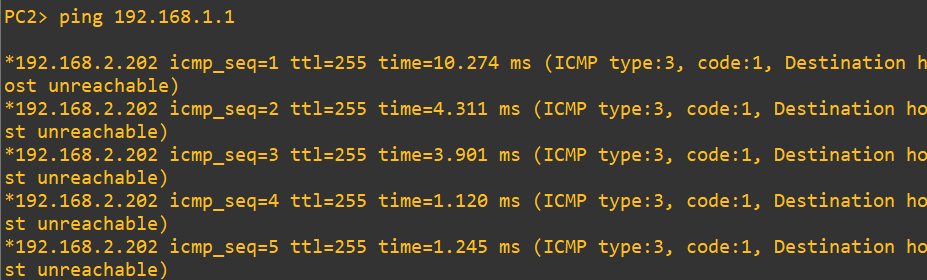
\includegraphics[width=0.7\textwidth]{pingPC2PC1SERIAL.png}
    \label{pingPC2PC1se}
\end{figure}


\chapter{Mission 2 - Route Discovery}

\section{Question - IPv6 compatibility}

\begin{questionBox}{IPv6 compatibility}
    From PC1, ping Router1 and PC2 IPv4 and IPv6 addresses. What is working ? Why ?    
\end{questionBox}



The results of the \textbf{trace} command for both PCs :

\begin{figure}[H]
    \caption{Traceroute from PC1 to PC2}
    \center
    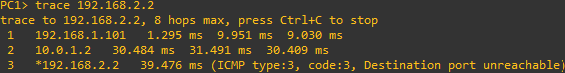
\includegraphics[width=0.7\textwidth]{tracePC1PC2.png}
    \label{tracepc1pc2}
\end{figure}

\begin{figure}[H]
    \caption{Traceroute from PC2 to PC1}
    \center
    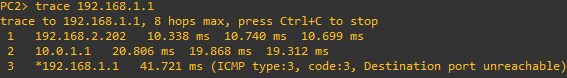
\includegraphics[width=0.7\textwidth]{tracePC2PC1.png}
    \label{tracepc2pc1}
\end{figure}

The routers R1 and R2 forms the path between both PCs. The length of this path is 2 (packets go through 2 routers).


\section{Question - How does Traceroute reveal the path between devices ?}

\begin{questionBox}{ How does Traceroute reveal the path between devices ?}
    By analysing carefully your trace command using Wireshark (do not hesitate to capture all the three links), you should be able to understand how it works. Explain in details how the traceroute command works (and interesting observations you can make). What are the layer 3 protocols used and why ?
\end{questionBox}


The traceroute command works as following :

\begin{enumerate}
    \item If the first router's IP address isn't already associated with a MAC address, first PC sends an ARP request.
    \item First PC sends an UDP packet to the destination with a source TTL (Time-To-Live) of 1.
    \item Packet arrives at the first router, decrements the source TTL by one : 1 $\rightarrow$ 0. If the TTL is zero, the router sends back an ICMP response (Time to live exceeded in transit) to the first PC.
    \item First PC resends an UDP packet to the destination but this time it increments the previous source TTL by one (1 $\rightarrow$ 2) so that the packet reaches the second router but not yet the destination. 
    \\ \textbf{Remark} : before incrementing the TTL, the first PC resends two times the packet (so at the end, three packets with TTL of 1 have been sent).
    \item And this goes on until the source TTL is high enough that the UDP packet arrives at the destination. When this happens, the destination PC sends an ICMP response (Port unreachable) to the first PC. Also the first step can be repeated at this stage but this time for the destination PC.
\end{enumerate}

\textbf{Observations} : 
\begin{itemize}
    \item Traceroute uses UDP and not TCP, this command doesn't search to establish a reliable connection (connectionless).
    \item Traceroute command is an iterative process. It starts from a very low TTL packet and stops when the TTL is enough. This is done for capturing the routers forming the path from source to destination.
    \item We can use the Traceroute command to test the latency for each node in the path.
\end{itemize}


There are 3 protocols from the layer 3 used in traceroute :

\begin{itemize}
    \item \textbf{ARP} or Address Resolution Protocol : it is used by the PCs to link the IP address to the MAC address of the routers they are directly connected to.
    \item \textbf{IPv4} : it is used for sending the UDP and ICMP packets from the source to the destination.
    \item \textbf{ICMP} : it is used for indicating the source that the TTL isn't high enough or indicating that the packet arrived at the destination.  
\end{itemize}

\begin{figure}[H]
    \caption{Traceroute from PC2 to PC1. Wireshark link between PC2 and R2}
    \center
    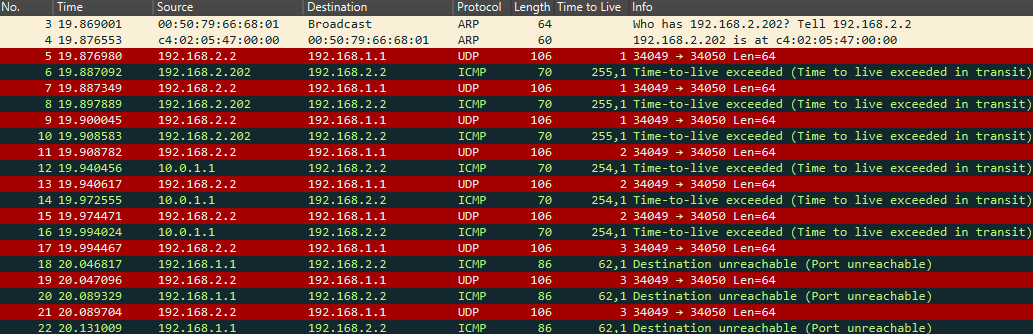
\includegraphics[width=0.7\textwidth]{traceroutePC2R2.png}
    \label{traceroutepc2r2}
\end{figure}

\begin{figure}[H]
    \caption{Traceroute from PC2 to PC1. Wireshark link between R2 and R1}
    \center
    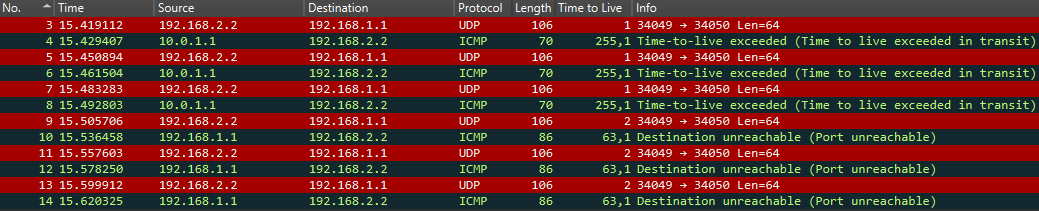
\includegraphics[width=0.7\textwidth]{tracerouteR2R1.png}
    \label{tracerouter2r1}
\end{figure}

\begin{figure}[H]
    \caption{Traceroute from PC2 to PC1. Wireshark link between R1 and PC1}
    \center
    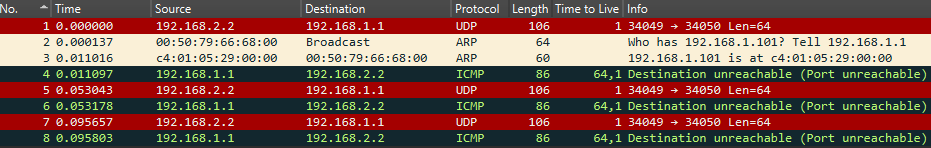
\includegraphics[width=0.7\textwidth]{tracerouteR1PC1.png}
    \label{tracerouter1pc1}
\end{figure}


\chapter{Mission 3 - Redundancy and dynamic re-routing}

\begin{figure}[H]
    \caption{New topology of the network}
    \center
    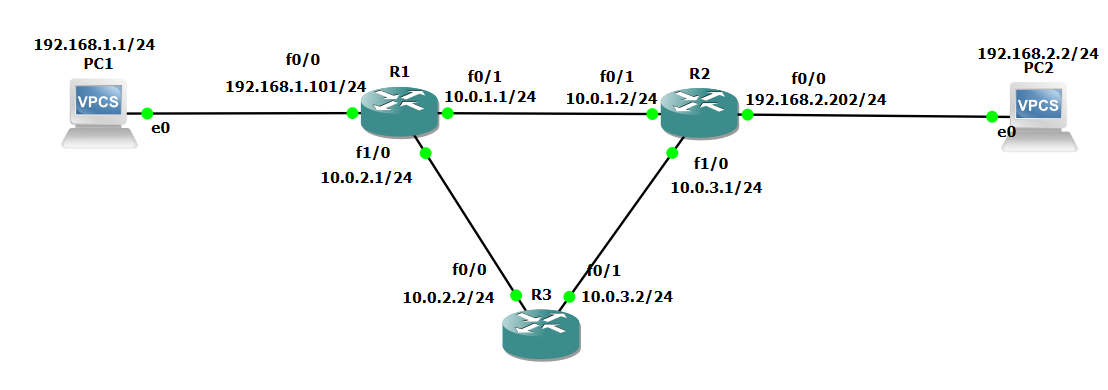
\includegraphics[width=0.7\textwidth]{topologyRRR.png}
    \label{newtopo}
\end{figure}


\section{Question - What is the route}

\begin{questionBox}{What is the route}
    What is the current route (IPs and devices) ? Did the route change (compared to mission 2: RIPv2) and why ?
\end{questionBox}

After adding a third router and configuring it, the route from PC1 to PC2 is (as seen in the figure \ref{tracePC1PC2rrr}) :

\begin{itemize}
    \item \textbf{PC1} (192.168.1.1) $\rightarrow$ \textbf{R1} (192.168.1.101) $\rightarrow$ \textbf{R2} (10.0.1.2) $\rightarrow$ \textbf{PC2} (192.168.2.2)  
\end{itemize}

This route is the same as in the mission 2, see figure \ref{tracepc1pc2}. It didn't change because it is the shortest route from PC1 to PC2. If the packets did go through the third router R3, it will take one more hop for the packets to arrive at PC2

\begin{figure}[H]
    \caption{Traceroute from PC1 to PC2 for the new topology}
    \center
    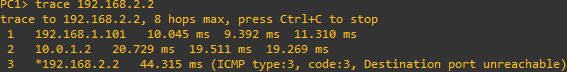
\includegraphics[width=0.7\textwidth]{tracePC1PC2RRR.png}
    \label{tracePC1PC2rrr}
\end{figure}




\section{Question - What changes in the routing table after a network link failure ?}

\begin{questionBox}{What changes in the routing table after a network link failure ?}
    Display the routing table of your routers. What have changed ? How much time has it taken to change ? What could happen if you do a ping between PC1 and PC2 before the changes takes place ? What is the current route and its length ? Did the route change and why ?
\end{questionBox}


The new routing tables for each router :

\begin{figure}[H]
    \caption{Routing table of R1 after updating the broken link}
    \center
    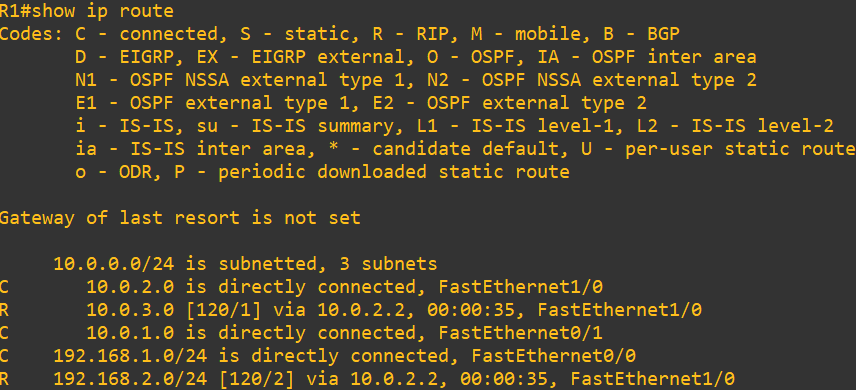
\includegraphics[width=0.7\textwidth]{routeR1down.png}
    \label{routedown1}
\end{figure}

\begin{figure}[H]
    \caption{Routing table of R2 after updating the broken link}
    \center
    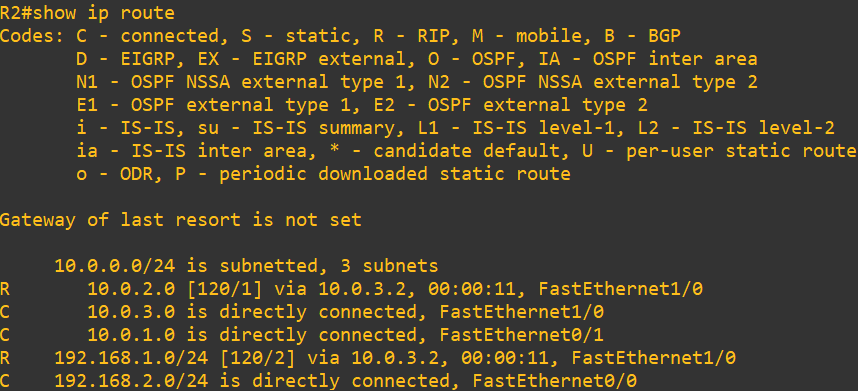
\includegraphics[width=0.7\textwidth]{routeR2down.png}
    \label{routedown2}
\end{figure}

\begin{figure}[H]
    \caption{Routing table of R3 after updating the broken link}
    \center
    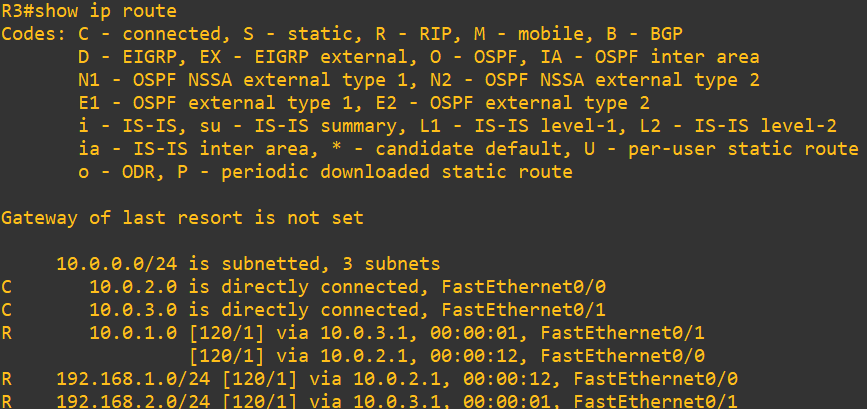
\includegraphics[width=0.7\textwidth]{routeR3dowb.png}
    \label{routedown3}
\end{figure}

Only two things have changed for the router R1 and R2 :

\begin{itemize}
    \item In order to access the subnet of the PCs, the routers now go through R3 (for example, R1 needs to take R3 to get to 192.168.2.0)
    \item There is now only one path to access the subnet between the routers and R3 (for example, before the change R1 could access 10.0.3.0 via R2 or R3)  
\end{itemize}


The change took approximately 260 seconds for R1 and for R2 after deleting the link in gns3.

\begin{figure}[H]
    \center
    \caption{Wireshark screenshots. Listening to link between R1 and R3. Bottom left shows RIPv2 content sent by R1. Deleted link around t=60 seconds}
    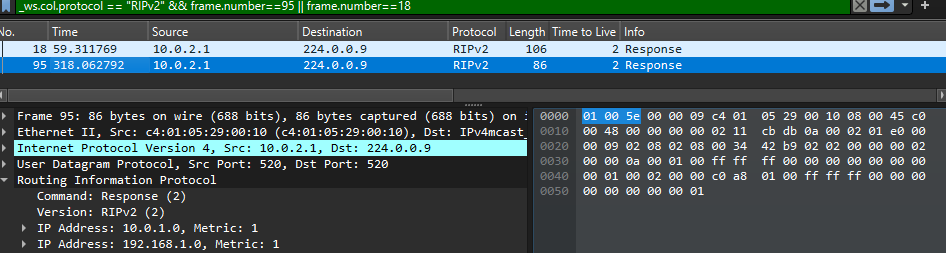
\includegraphics[width=0.7\textwidth]{routetablechange.png}
    \label{routchange}
\end{figure}
\begin{figure}[H]
    \caption{Wireshark screenshots. Listening to link between R2 and R3. Bottom left shows RIPv2 content sent by R2. Deleted link around t=60 seconds}
    \center
    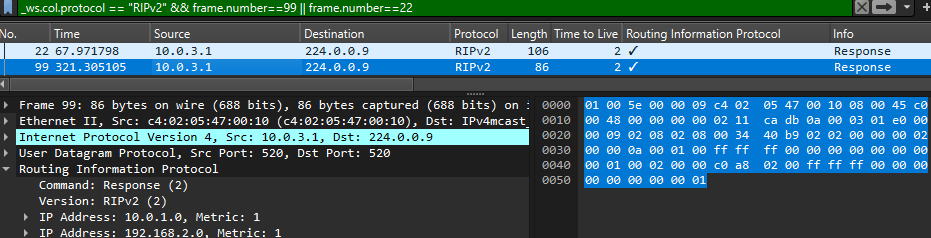
\includegraphics[width=0.7\textwidth]{routetablechange2.png}
    \label{routchange2}
\end{figure}

The current path is the following (inverse for PC2 to PC1) with length three (packets go through 3 routers):

\begin{figure}[H]
    \caption{Trace command from PC1 to PC2}
    \center
    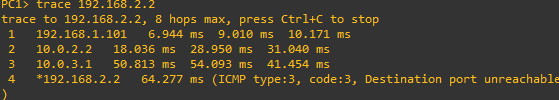
\includegraphics[width=0.7\textwidth]{tracepc1pc2down.png}
    \label{tracedown}
\end{figure}

\begin{itemize}
    \item \textbf{PC1} $\rightarrow$ \textbf{R1} (192.168.1.101) $\rightarrow$ \textbf{R3} (10.0.2.2) $\rightarrow$ \textbf{R2} (10.0.3.1) $\rightarrow$ \textbf{PC2} (192.168.2.2)
\end{itemize}

As we can see, the route did in fact change after the link between R1 and R2 has been broken. The RIP updated the routing table of each router after the destruction of the link

If we do a ping between PC1 and PC2 before the changes take place, we have no response from PC2 (see figure \ref{routepc1pc2broke}) because the first router didn't update the routing table and tries to send the packets through the broken link. We can see more clearly with the trace command (figure \ref{tracepc1pc2broke}) that we don't get an answer from R2.

\begin{figure}[H]
    \caption{Ping from PC1 to PC2 with broken link and no changes in routing tables}
    \center
    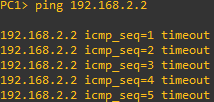
\includegraphics[scale=0.8]{pingPC1PC2broke.png}
    \label{routepc1pc2broke}
\end{figure}

\begin{figure}[H]
    \caption{Trace from PC1 to PC2 with broken link and no changes in routing tables}
    \center
    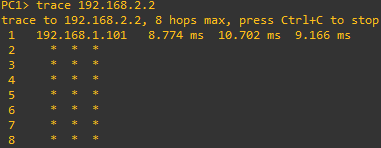
\includegraphics[scale=0.8]{tracePC1PC2broke.png}
    \label{tracepc1pc2broke}
\end{figure}

\section{Bonus question - VPN Security}

\begin{bonusQuestionBox}{VPN Security}
    Is VPN really a good way to secure your communication ? Why ? If it is not the case, what could you do instead (or in addition) ?
\end{bonusQuestionBox}


The routers don't send the part of the routing tables that corresponds to a network which is directly connected to another router. For example, R3 doesn't tell R1 that it can serve the networks 192.168.1.0/24 and 10.0.1.0/24 because R1 is directly connected to these networks. However, R3 tells R1 that it is serving the networks 10.0.3.0/24 and 192.168.2.0/24.

Remark : routers don't send the network with which they communicate (in the previous case, neither R1 or R3 send to each other the fact that they serve the network 10.0.2.0, it is the subnet that connects them)

Why the routers do that ? The routers don't send these parts because the metrics associated with these networks will be always higher than the metric for a router direclty connected to it. 
\\ In fact, it is rather the router that is directly connected to a subnet that advertises it to other routers. The goal is to set up the shortest path from one network to another.

\begin{figure}[H]
    \caption{Wireshark screenshot. Listening to link between R1 and R3. Bottom left shows RIPv2 content sent from R3}
    \center
    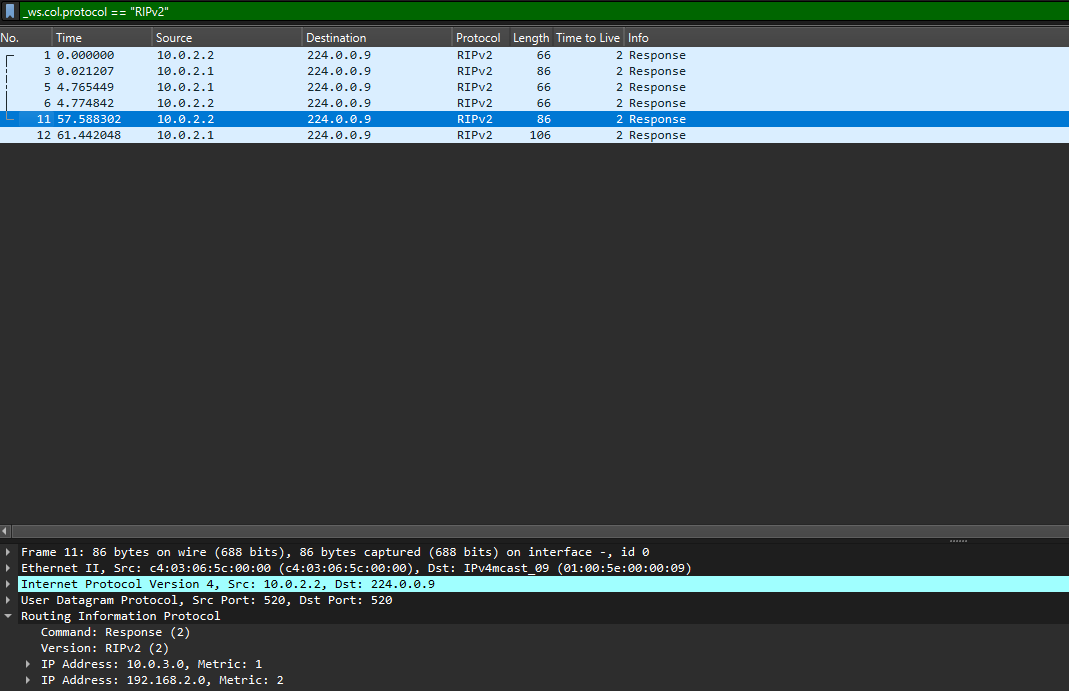
\includegraphics[width=0.7\textwidth]{wiresharkRIPRRR.png}
    \label{riprrr}
\end{figure}

\begin{figure}[H]
    \caption{Wireshark screenshot. Listening to link between R1 and R3. Bottom left shows RIPv2 content sent from R1}
    \center
    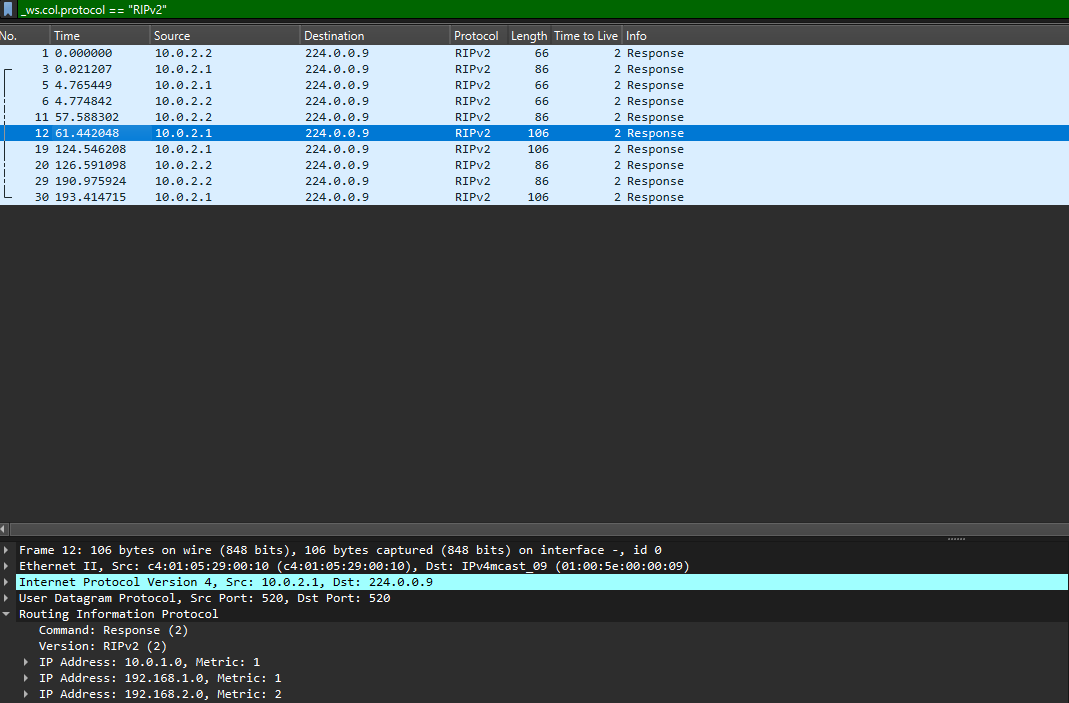
\includegraphics[width=0.7\textwidth]{wiresharkRIPRRR_2.png}
    \label{riprrr2}
\end{figure}


\end{document}	

